\chapter{Cơ sở lý thuyết và các nghiên cứu liên quan}
\label{ch:co-so-ly-thuyet}

Chương này trình bày cơ sở lý thuyết y sinh học và phương pháp luận học máy nền tảng cho bài toán dự đoán mức độ triệu chứng trầm cảm từ dữ liệu sinh lý dạng bảng, đồng thời khảo sát có hệ thống các công trình nghiên cứu tiền nhiệm. Nội dung chương tập trung vào: (1) Cấu trúc thang đo chuẩn PHQ-9 và các cơ chế sinh học kết nối chỉ số cận lâm sàng với triệu chứng trầm cảm; (2) Hai thách thức bản chất của dữ liệu y tế dạng bảng gồm mất cân bằng lớp cực đoan và chồng lấn phân phối đặc trưng; (3) Ba trường phái mô hình hóa gồm phân loại phẳng, phân loại phân cấp kết hợp lý thuyết quyết định nhạy chi phí Bayes, và phân loại thứ bậc; (4) Tổng hợp các nghiên cứu liên quan nhằm định vị rõ khoảng trống học thuật mà đề tài giải quyết.

\section{Thang đo PHQ-9 và cơ sở sinh lý học của triệu chứng trầm cảm}
\label{sec:thang-do-phq9-va-sinh-ly}

\subsection{Cấu trúc thang đo PHQ-9 và lượng hóa lâm sàng}
\label{subsec:cau-truc-phq9}

Thang đo Sức khỏe Bệnh nhân 9 mục (Patient Health Questionnaire-9 -- PHQ-9) là một cấu phần chẩn đoán tâm thần tiêu chuẩn hóa, do Kroenke, Spitzer và Williams phát triển \cite{kroenke2001phq, spitzer1999validation}. PHQ-9 gồm 9 mục tự báo cáo phản ánh tần suất xuất hiện các triệu chứng trong vòng hai tuần gần nhất, tương ứng với tiêu chuẩn DSM-IV:
\begin{enumerate}
    \item Giảm sự hứng thú hoặc niềm vui trong các hoạt động hàng ngày (Anhedonia).
    \item Cảm giác buồn bã, chán nản, u sầu hoặc tuyệt vọng (Depressed mood).
    \item Rối loạn giấc ngủ: khó ngủ, mất ngủ hoặc ngủ quá nhiều (Sleep disturbance).
    \item Cảm giác kiệt sức, mệt mỏi hoặc thiếu năng lượng (Fatigue).
    \item Rối loạn cảm giác thèm ăn: chán ăn hoặc ăn quá mức (Appetite changes).
    \item Cảm giác thất bại, tự ti hoặc mặc cảm tội lỗi (Feelings of worthlessness).
    \item Giảm khả năng tập trung chú ý khi làm việc hoặc sinh hoạt (Concentration problems).
    \item Chậm chạp vận động hoặc kích động, bồn chồn (Psychomotor changes).
    \item Suy nghĩ về cái chết hoặc ý định tự gây thương tích (Suicidal ideation).
\end{enumerate}

Mỗi mục được chấm điểm theo thang Likert 4 mức độ từ 0 đến 3 (0: Hoàn toàn không; 1: Vài ngày; 2: Hơn một nửa số ngày; 3: Gần như mỗi ngày). Tổng điểm số $s = \sum_{j=1}^9 \text{DPQ}_j \in [0, 27]$ được ánh xạ thành 5 mức độ nghiêm trọng lâm sàng chuẩn được minh họa trong Hình \ref{fig:phq9-tiers}.

\begin{figure}[htbp]{Thang đo PHQ-9 (0--27 điểm), 5 bậc nghiêm trọng lâm sàng và ánh xạ sang không gian 3 nhóm $T_3$}
\centering
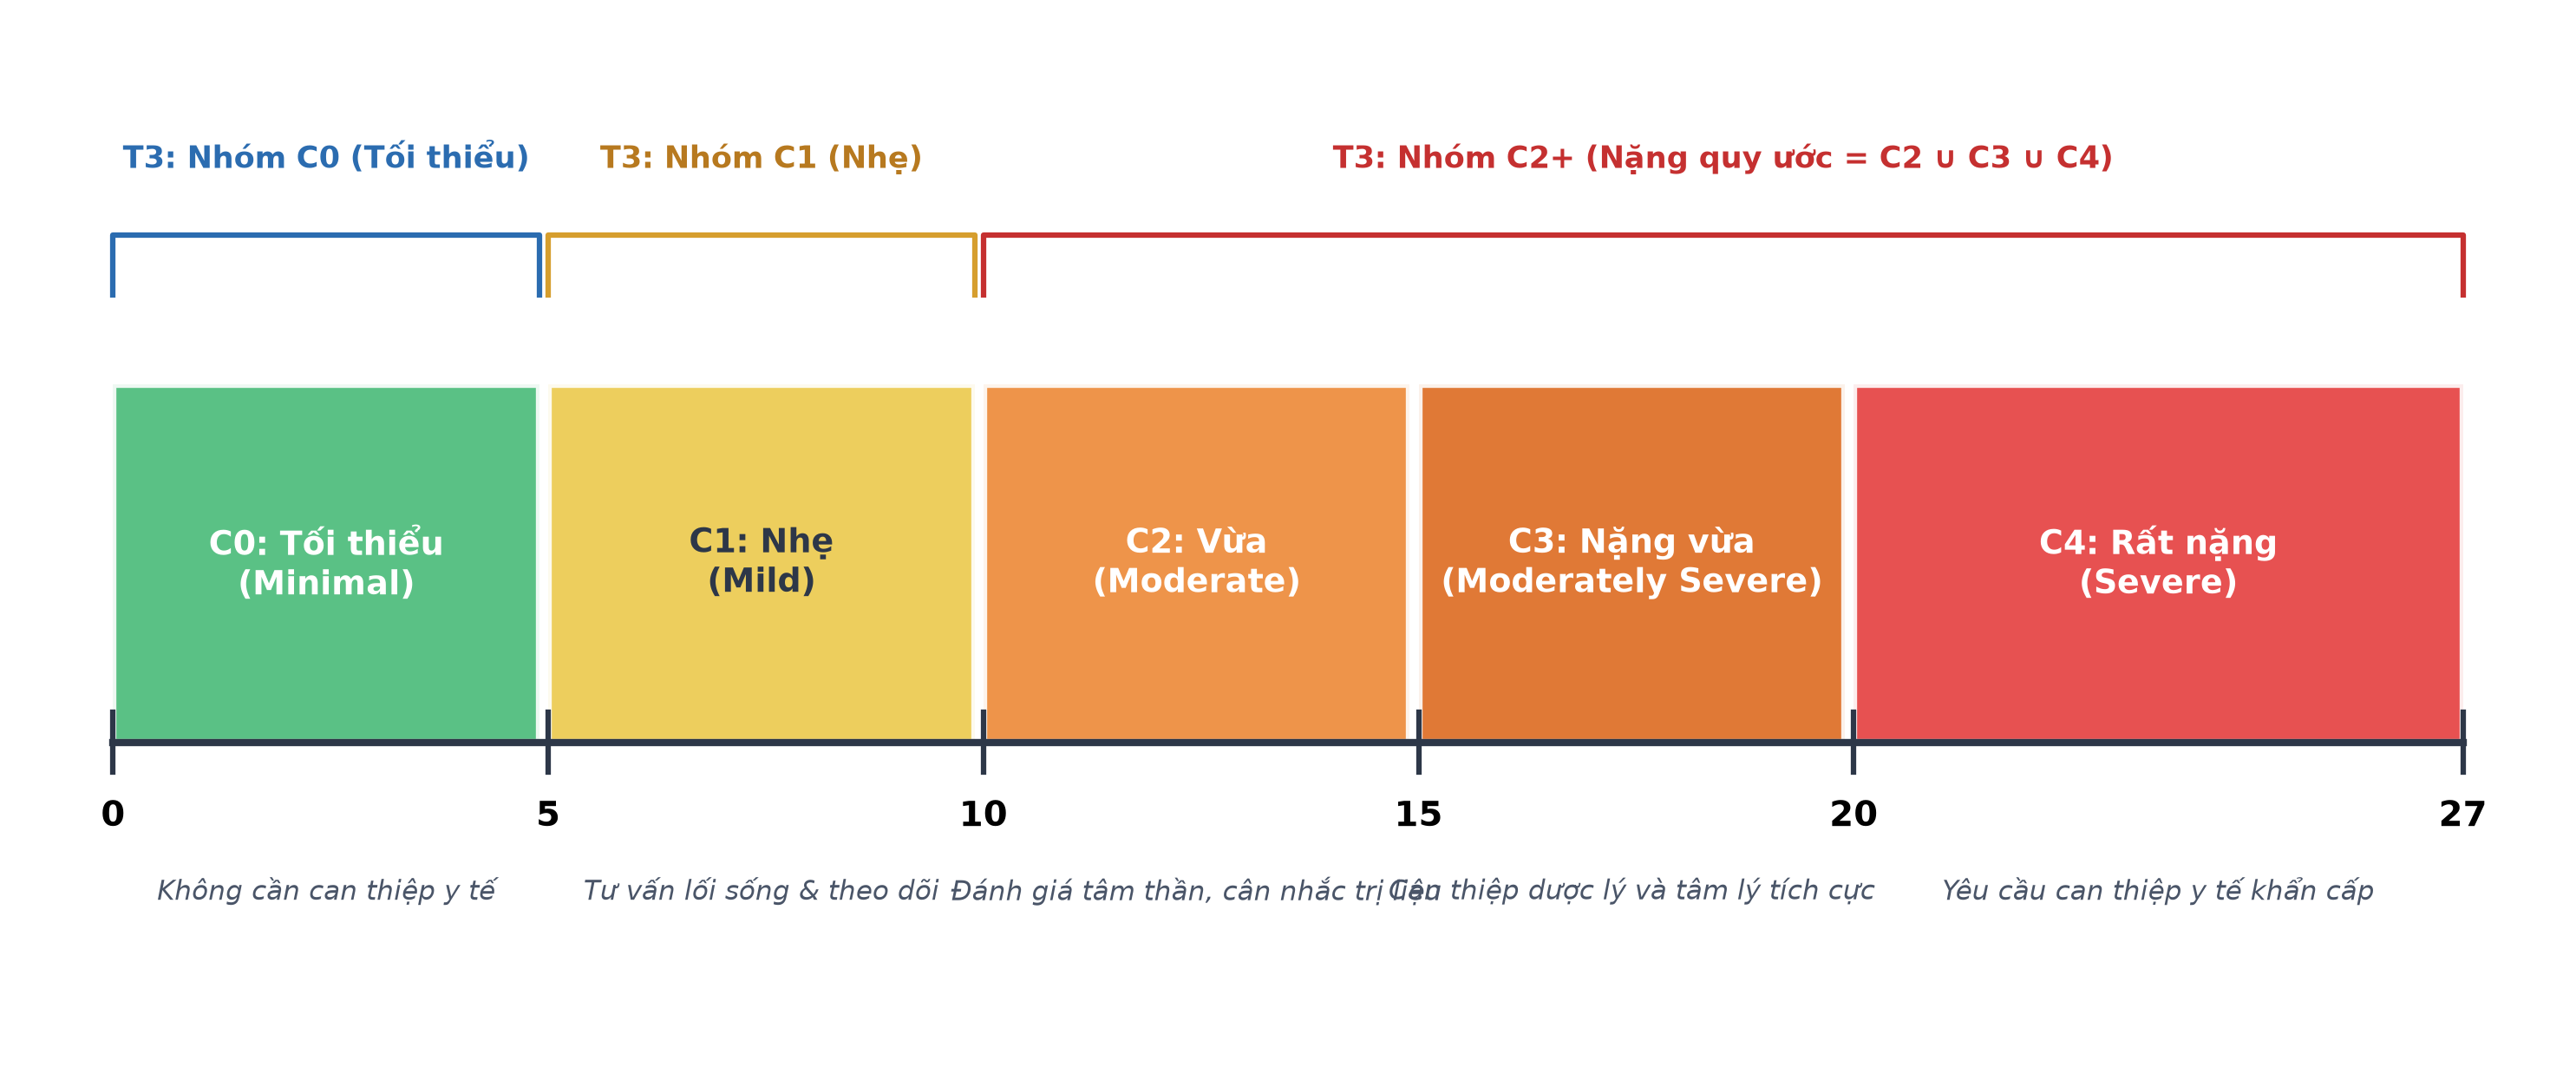
\includegraphics[width=\textwidth]{figures/fig2_phq9_tiers.png}
\label{fig:phq9-tiers}
\end{figure}
\FloatBarrier

Theo quy ước quốc tế:
\begin{itemize}
    \item $s \in [0, 4]$ ($C_0$ -- Tối thiểu): Trạng thái bình thường, không yêu cầu can thiệp y tế.
    \item $s \in [5, 9]$ ($C_1$ -- Nhẹ): Xuất hiện triệu chứng cận lâm sàng, khuyến nghị theo dõi và tư vấn tâm lý lối sống.
    \item $s \in [10, 14]$ ($C_2$ -- Vừa): Ngưỡng cắt lâm sàng bắt đầu điều trị, cần bác sĩ chuyên khoa đánh giá.
    \item $s \in [15, 19]$ ($C_3$ -- Nặng vừa): Cần can thiệp tích cực kết hợp liệu pháp dược lý và tâm lý.
    \item $s \in [20, 27]$ ($C_4$ -- Rất nặng): Yêu cầu can thiệp khẩn cấp chuyên khoa tâm thần.
\end{itemize}

Trong khuôn khổ đề tài DepSev-ML, bên cạnh không gian 5 bậc tiêu chuẩn ($T_5$), bài toán còn được khảo sát trên không gian 3 nhóm gộp quy ước ($T_3$), trong đó nhóm $C_2^+$ đại diện cho toàn bộ các đối tượng có triệu chứng từ mức Vừa đến Rất nặng ($C_2 \cup C_3 \cup C_4$, tương ứng $s \ge 10$).

\subsection{Cơ sở sinh lý học và các chỉ dấu y sinh học}
\label{subsec:co-so-sinh-ly}

Mặc dù triệu chứng trầm cảm thể hiện qua cảm xúc và hành vi, các nghiên cứu y sinh học hiện đại đã chứng minh trầm cảm là một bệnh lý toàn thân có tương tác mật thiết với các rối loạn sinh hóa và chuyển hóa ngoại vi thông qua trục não-ruột, hệ thống miễn dịch và trục hạ đồi-tuyến yên-tuyến thượng thận (HPA) \cite{pratt1991discriminant}.

\begin{figure}[htbp]{Các cơ chế y sinh học liên kết chỉ số sinh lý ngoại vi với mức độ triệu chứng trầm cảm}
\centering
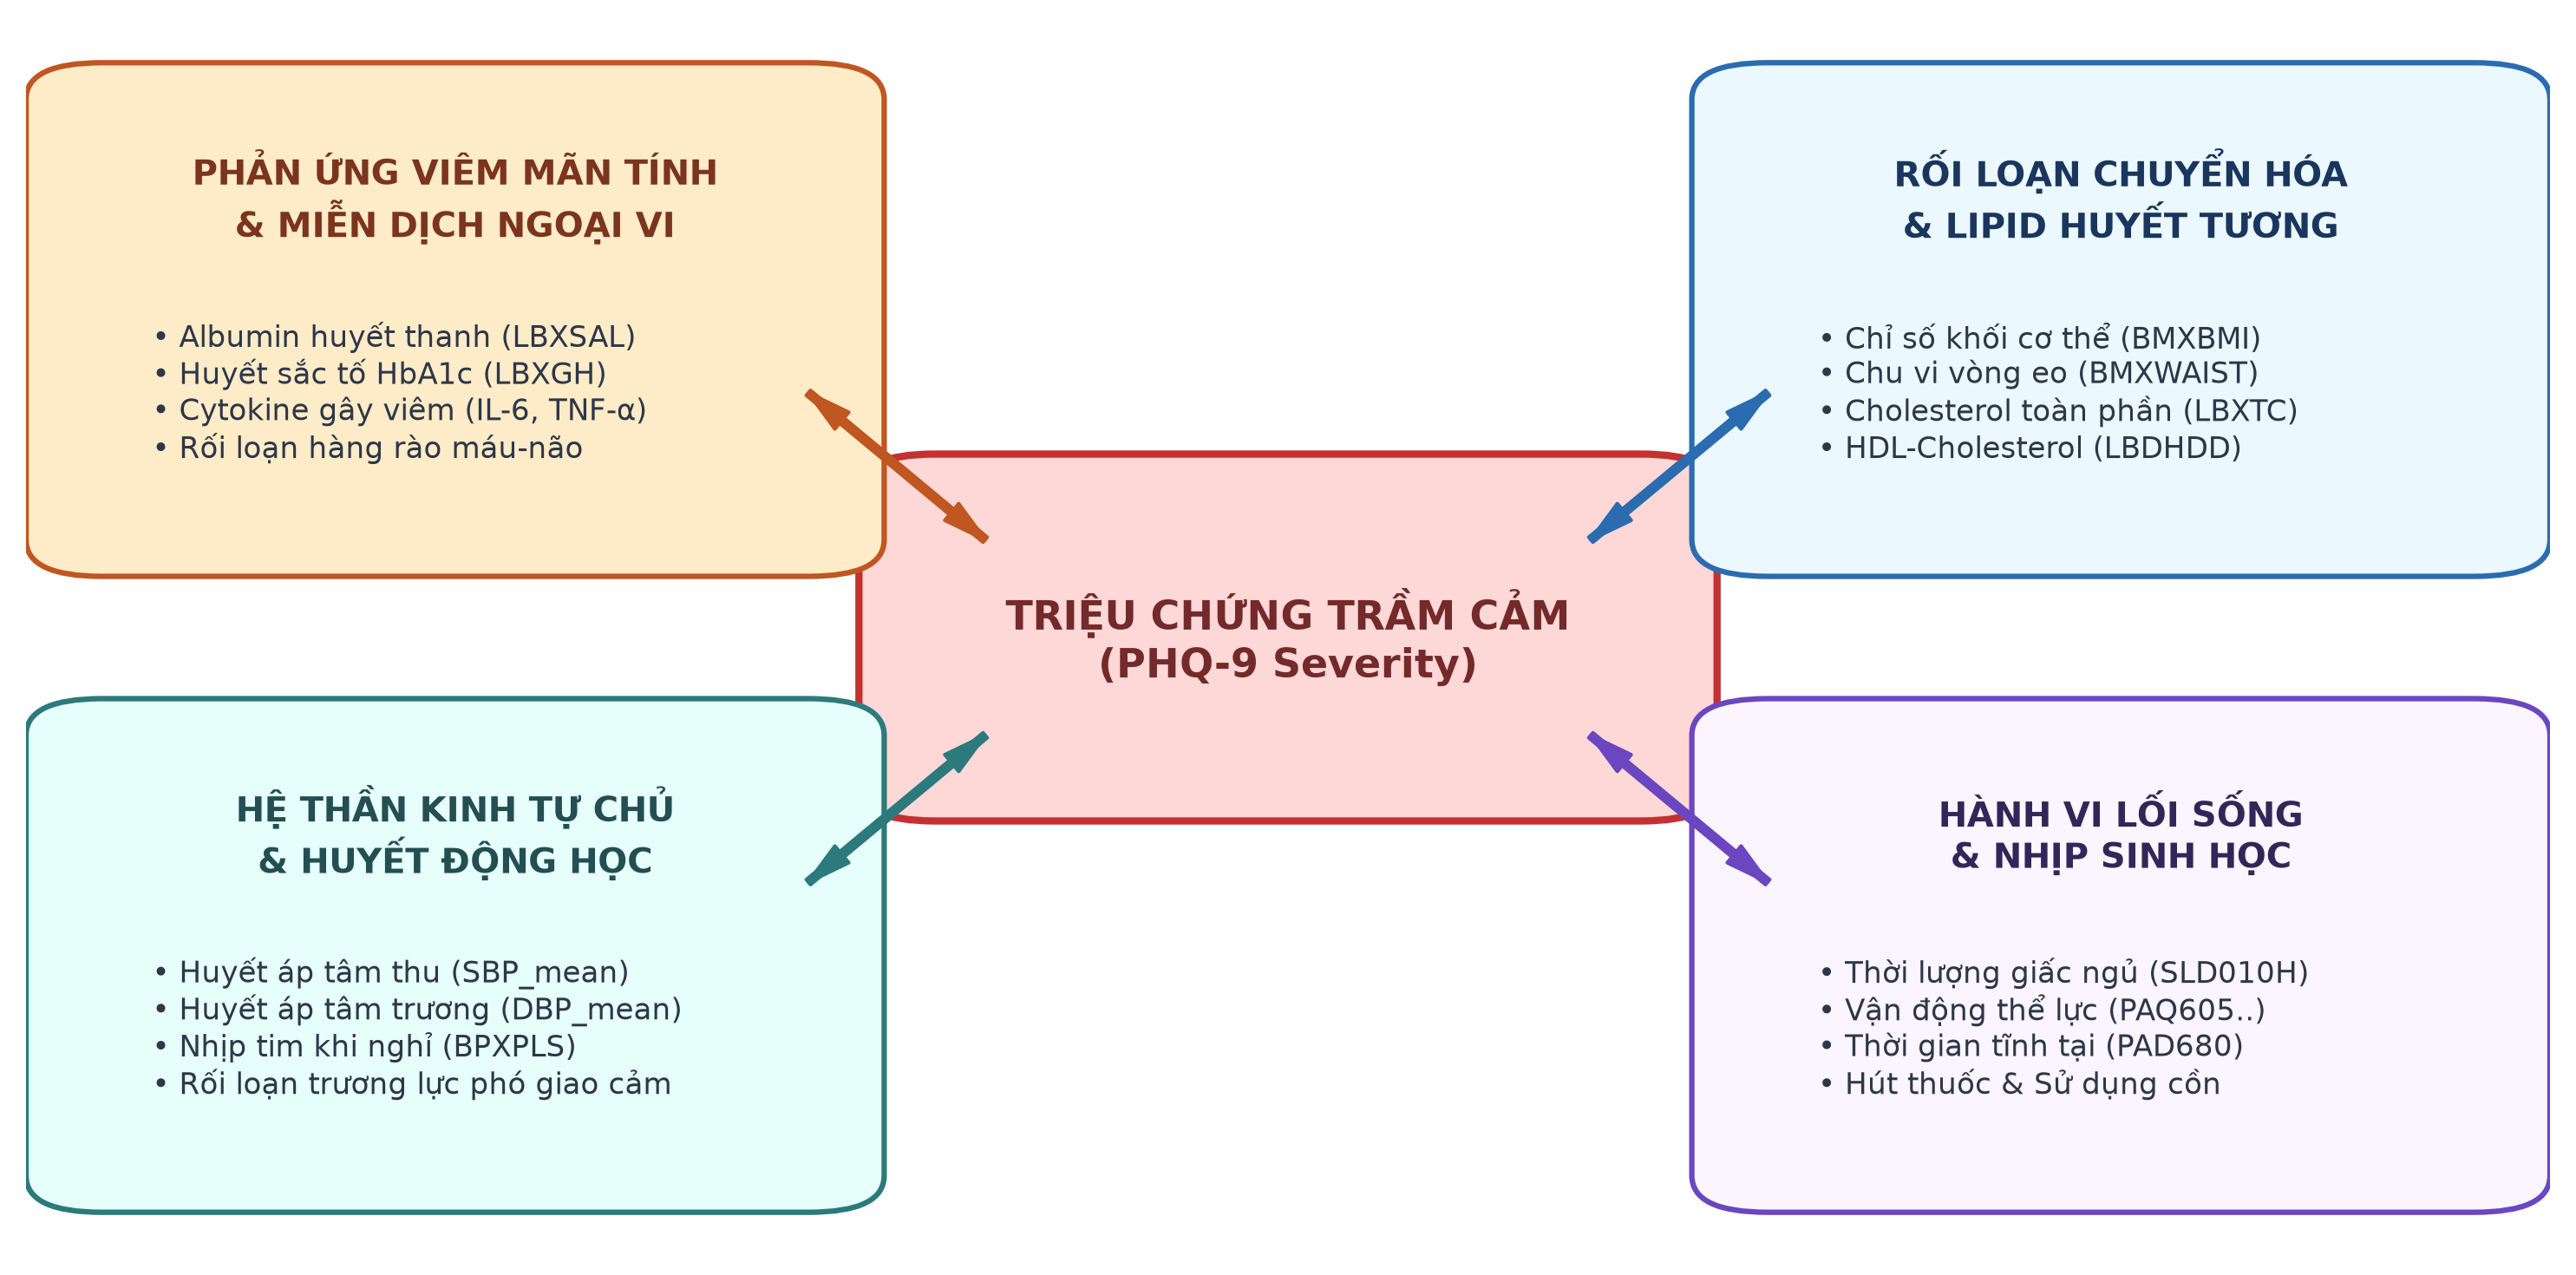
\includegraphics[width=\textwidth]{figures/fig2_gut_brain_metabolic_axis.png}
\label{fig:gut-brain-axis}
\end{figure}
\FloatBarrier

Như mô tả trong Hình \ref{fig:gut-brain-axis}, các nhóm biến số ngoại vi trong NHANES phản ánh bốn cơ chế bệnh sinh chính:
\begin{enumerate}
    \item \textbf{Phản ứng viêm mãn tính thể nhẹ và miễn dịch ngoại vi:} Trầm cảm kích hoạt các cytokine gây viêm ngoại vi (IL-6, TNF-$\alpha$). Nồng độ Albumin huyết thanh (LBXSAL) phản ánh tình trạng dinh dưỡng và là protein điều biến phản ứng viêm âm tính; trong khi chỉ số đường huyết tích lũy Glycohemoglobin HbA1c (LBXGH) phản ánh mức độ căng thẳng oxy hóa và kháng insulin.
    \item \textbf{Rối loạn chuyển hóa và lipid huyết tương:} Sự rối loạn hoạt động chuyển hóa thể hiện rõ qua các chỉ số nhân trắc học như chỉ số khối cơ thể (BMXBMI), chu vi vòng eo (BMXWAIST), kết hợp cùng nồng độ Cholesterol toàn phần (LBXTC) và HDL-Cholesterol bảo vệ tim mạch (LBDHDD).
    \item \textbf{Hệ thần kinh tự chủ và huyết động học:} Sự mất cân bằng giữa trương lực giao cảm và phó giao cảm dẫn đến biến đổi nhịp tim khi nghỉ (BPXPLS), huyết áp tâm thu (SBP\_mean) và huyết áp tâm trương (DBP\_mean).
    \item \textbf{Hành vi lối sống và nhịp sinh học:} Giấc ngủ suy giảm (SLD010H), mức độ hoạt động thể lực thấp (PAQ605..), thời gian ngồi tĩnh tại kéo dài (PAD680) cùng với hành vi sử dụng chất kích thích (hút thuốc, rượu bia) có mối quan hệ nhân quả hai chiều với sự gia tăng triệu chứng trầm cảm.
\end{enumerate}

\section{Đặc thù và thách thức của dữ liệu y tế dạng bảng}
\label{sec:dac-thu-du-lieu-bang}

Dữ liệu y tế dạng bảng trích xuất từ các khảo sát cộng đồng như NHANES có những đặc thù hình học phức tạp, khác biệt căn bản so với dữ liệu thị giác máy tính hay xử lý ngôn ngữ tự nhiên.

\subsection{Mất cân bằng lớp cực đoan (Severe Class Imbalance)}
\label{subsec:mat-can-bang-lop}

Trong các cuộc điều tra dịch tễ quy mô quốc gia, tỷ lệ mắc các bệnh lý tâm thần mức độ nghiêm trọng luôn chiếm thiểu số. Giả sử tập dữ liệu có $K$ lớp với kích thước $N_0, N_1, \dots, N_{K-1}$, tỷ số mất cân bằng (Imbalance Ratio -- IR) được định nghĩa bởi:
\begin{equation}
    \text{IR} = \frac{\max_k N_k}{\min_k N_k}
\end{equation}
Trong tập dữ liệu phát triển Legacy của đề tài ($N = 4.045$), lớp $C_0$ chiếm tới $3.016$ đối tượng (74.56\%), trong khi lớp rất nặng $C_4$ chỉ có $44$ đối tượng (1.09\%), tạo nên tỷ số mất cân bằng lên tới $\text{IR} = 3016 / 44 \approx 68.5:1$ (Hình \ref{fig:imbalance-overlap}a).

Nếu mô hình học máy được huấn luyện nhằm tối thiểu hóa sai số toàn cục (hoặc hàm mất mát Cross-Entropy tiêu chuẩn), thuật toán sẽ bị thiên lệch mạnh về phía lớp $C_0$, dẫn tới hiện tượng đạt độ chính xác Accuracy rất cao nhưng hoàn toàn bỏ sót các ca bệnh thực tế. Để khắc phục hiện tượng này, kỹ thuật gán trọng số nghịch đảo tần số lớp (Class-weighted objective) được áp dụng:
\begin{equation}
    w_k = \frac{N}{K \cdot N_k}
\end{equation}
giúp cân bằng lại đóng góp của các mẫu thuộc lớp hiếm vào đạo hàm hàm mất mát.

\begin{figure}[htbp]{(a) Mất cân bằng lớp cực đoan trên tập dữ liệu và (b) Hiện tượng chồng lấn phân phối đặc trưng sinh lý}
\centering
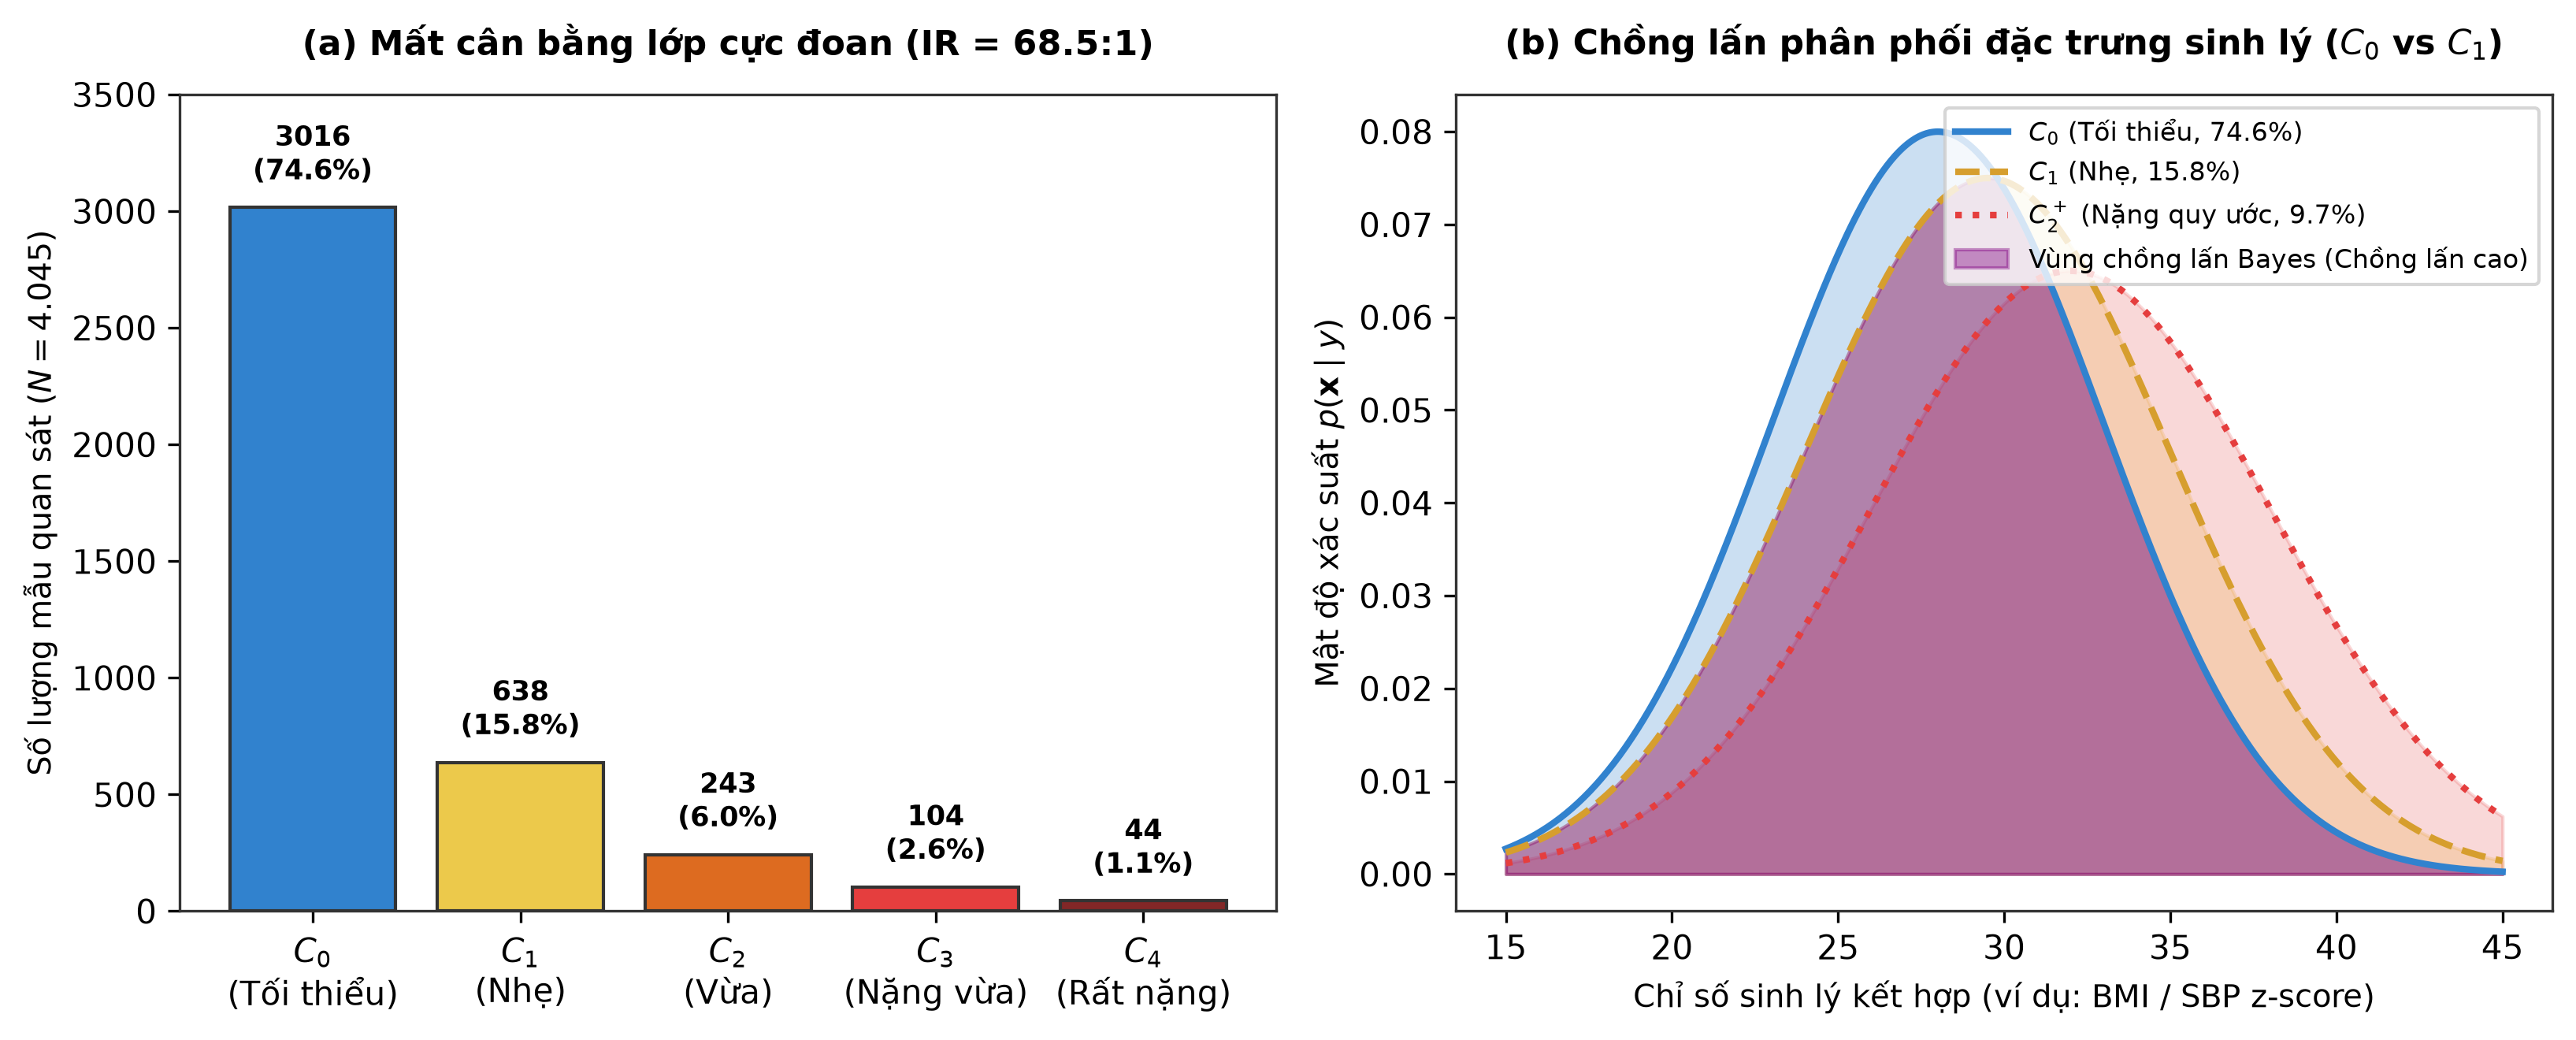
\includegraphics[width=\textwidth]{figures/fig2_imbalance_overlap.png}
\label{fig:imbalance-overlap}
\end{figure}
\FloatBarrier

\subsection{Chồng lấn phân phối đặc trưng (Feature Overlap)}
\label{subsec:chong-lan-dac-trung}

Khác với các xét nghiệm chẩn đoán đặc hiệu (chẳng hạn như kháng nguyên ung thư hay xét nghiệm virus), các chỉ số sinh lý như huyết áp, cholesterol hay BMI không có một ngưỡng cắt sinh học duy nhất để phân tách người bình thường và người có triệu chứng trầm cảm. Phân phối xác suất điều kiện của đặc trưng $\mathbf{x}$ giữa hai trạng thái kế cận $p(\mathbf{x} \mid Y = 0)$ và $p(\mathbf{x} \mid Y = 1)$ có diện tích giao thoa rất lớn (Hình \ref{fig:imbalance-overlap}b).

Vùng lỗi Bayes tối thiểu (Bayes Error Region) được xác định bởi:
\begin{equation}
    \Omega_{\text{overlap}} = \int \min\left(P(Y=0)p(\mathbf{x} \mid Y=0), P(Y=1)p(\mathbf{x} \mid Y=1)\right) d\mathbf{x}
\end{equation}
Khi $\Omega_{\text{overlap}}$ lớn, kể cả bộ phân loại tối ưu lý thuyết cũng không thể đạt được độ chính xác tuyệt đối. Do đó, việc cải thiện hiệu năng không thể chỉ dựa vào việc chọn thuật toán phức tạp hơn mà bắt buộc phải khai thác các kiến trúc phân loại phù hợp và kiểm soát chặt chẽ sự đánh đổi lâm sàng.

\section{Các trường phái mô hình hóa trong bài toán phân loại thứ bậc}
\label{sec:truong-phai-mo-hinh-hoa}

Để xử lý bài toán phân tầng nguy cơ trầm cảm, nghiên cứu khảo sát và so sánh ba trường phái mô hình hóa chính được minh họa trong Hình \ref{fig:modeling-paradigms}.

\begin{figure}[htbp]{Ba trường phái mô hình hóa: (a) Phân loại phẳng, (b) Phân loại phân cấp hai giai đoạn, và (c) Phân loại thứ bậc}
\centering
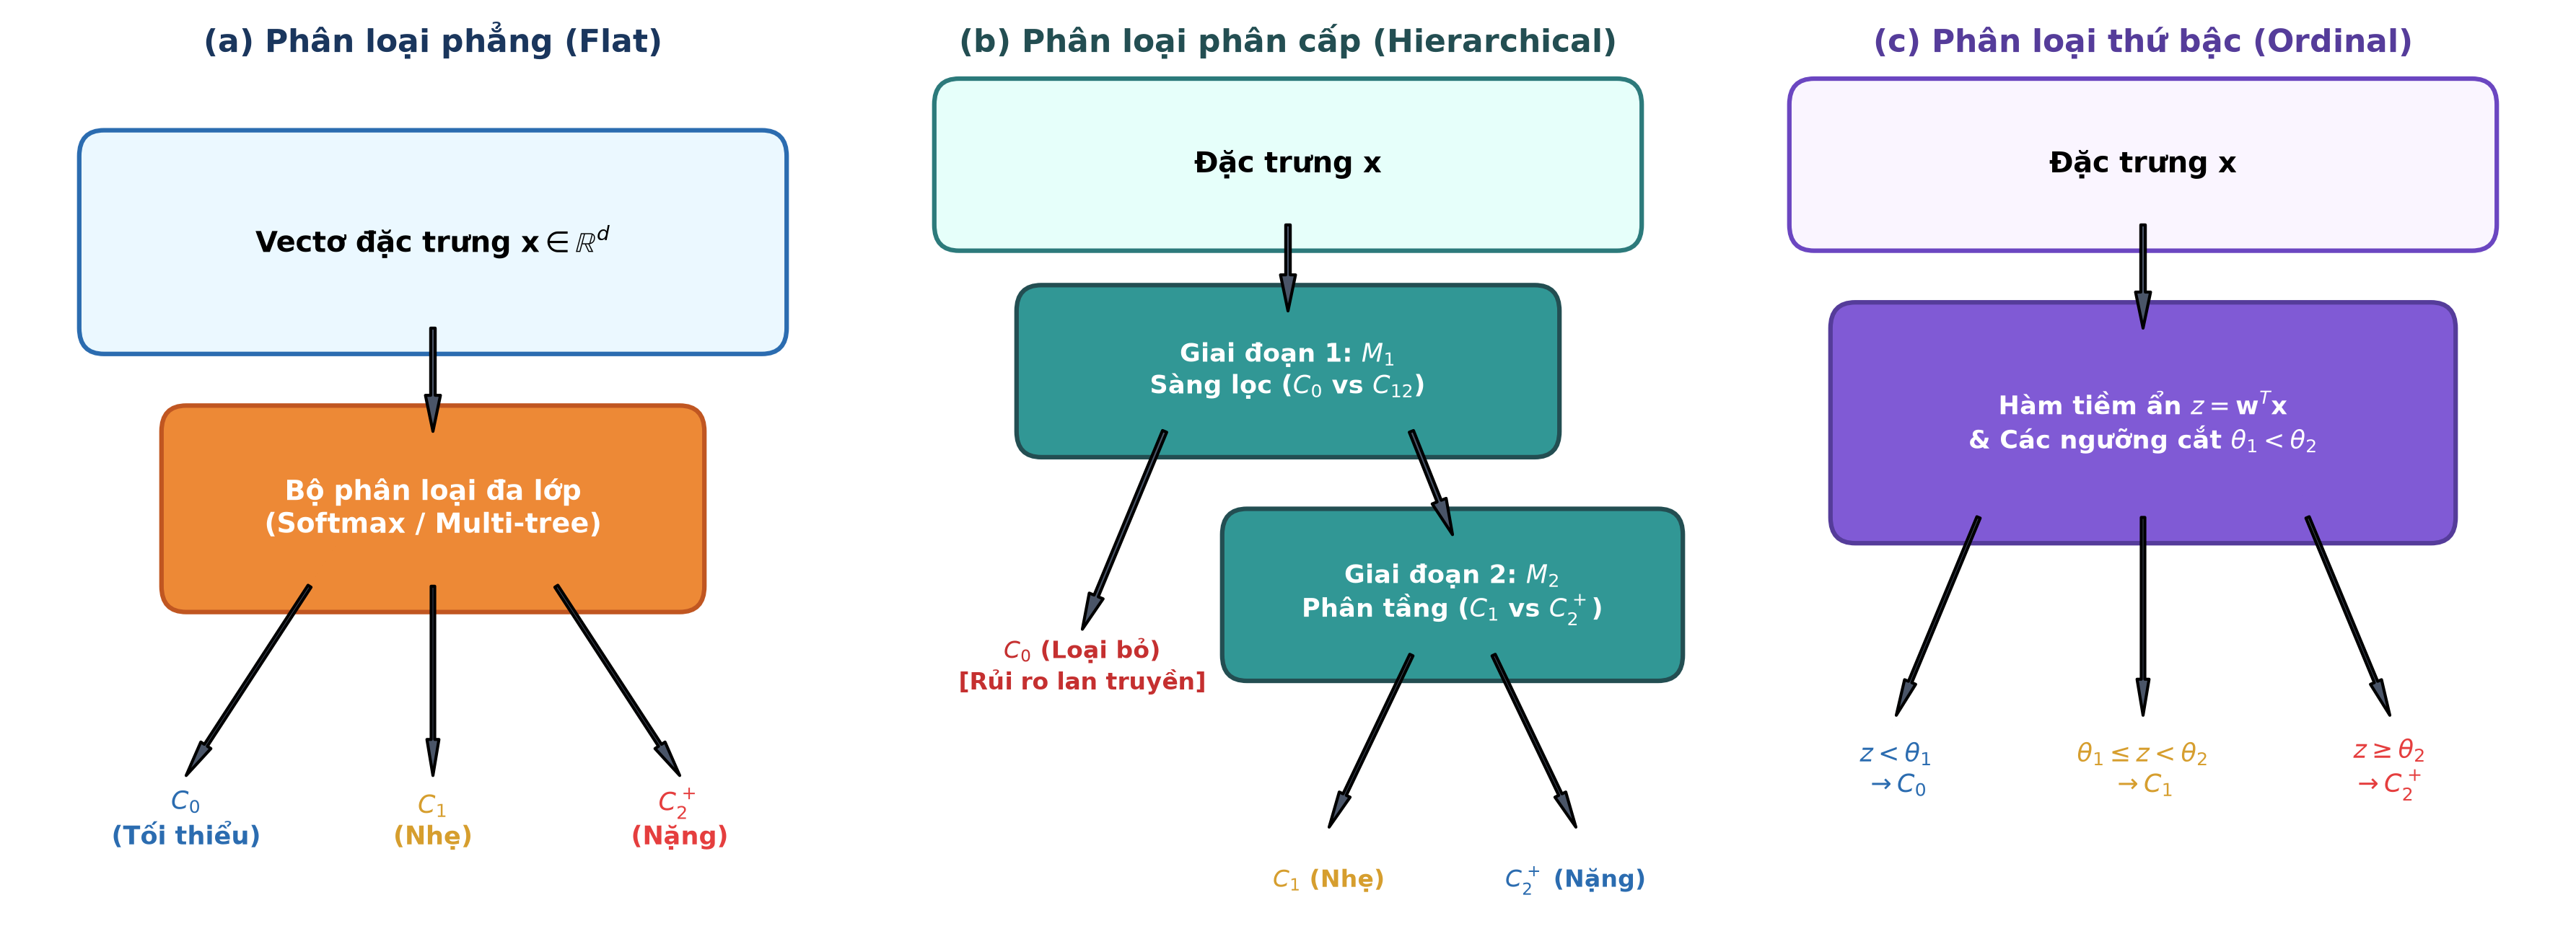
\includegraphics[width=\textwidth]{figures/fig2_modeling_paradigms.png}
\label{fig:modeling-paradigms}
\end{figure}
\FloatBarrier

\subsection{Trường phái phân loại phẳng (Flat Classification)}
\label{subsec:flat-paradigm}

Cách tiếp cận phân loại phẳng coi $K$ mức độ nghiêm trọng là các nhãn danh nghĩa (nominal classes) hoàn toàn độc lập. Mô hình học trực tiếp một hàm ánh xạ $f: \mathbb{R}^d \to \Delta^K$ để dự đoán phân phối xác suất hậu nghiệm $P(Y = k \mid \mathbf{x})$. Các thuật toán phổ biến bao gồm Hồi quy Logistic đa thức, Rừng ngẫu nhiên (Random Forest) và Tăng cường độ dốc cực đại (XGBoost).

Hạn chế căn bản của trường phái phân loại phẳng là bỏ qua hoàn toàn quan hệ thứ bậc tự nhiên giữa các mức độ ($C_0 < C_1 < C_2$). Một sai lầm nhầm lẫn giữa $C_0$ và $C_1$ (cách nhau 1 bậc) bị hàm mất mát đối xử tương đương như sai lầm cực kỳ nguy hiểm giữa $C_0$ và $C_2^+$ (cách nhau 2 bậc). Đồng thời, khi dữ liệu bị mất cân bằng trầm trọng, các ranh giới phân tách phẳng dễ bị đẩy ép về phía các lớp thiểu số.

\subsection{Trường phái phân loại phân cấp (Hierarchical Classification)}
\label{subsec:hierarchical-paradigm}

Nhằm mô phỏng quy trình sàng lọc lâm sàng thực tế của bác sĩ (trước hết xác định người đó có triệu chứng hay không, sau đó mới đánh giá mức độ nặng), trường phái phân cấp chia nhỏ bài toán phức tạp thành một cấu trúc cây gồm hai giai đoạn \cite{silla2011survey}:
\begin{itemize}
    \item \textbf{Giai đoạn 1 (Bộ phân loại sàng lọc $M_1$):} Phân loại nhị phân giữa nhóm không có triệu chứng ($C_0$) và nhóm có triệu chứng ($C_{12} = C_1 \cup C_2^+$).
    \item \textbf{Giai đoạn 2 (Bộ phân loại phân tầng $M_2$):} Tiếp nhận các đối tượng được xác định có triệu chứng để phân biệt giữa mức độ nhẹ ($C_1$) và mức độ nặng ($C_2^+$).
\end{itemize}

Tuy nhiên, trong triển khai thực tế, kiến trúc phân cấp chia làm hai cơ chế định tuyến khác nhau:
\begin{enumerate}
    \item \textbf{Định tuyến cứng (Hard Routing):} Nếu $M_1$ dự đoán một mẫu là $C_0$, mẫu đó lập tức bị loại bỏ khỏi luồng xử lý và không bao giờ được $M_2$ xem xét. Cơ chế này dẫn đến hiện tượng \textbf{lan truyền sai số một chiều (Error Propagation)}: nếu một ca bệnh nặng $C_2^+$ bị $M_1$ gán nhầm thành $C_0$, sai sót này sẽ bị khóa vĩnh viễn và biến thành lỗi nghiêm trọng nhất trong y khoa.
    \item \textbf{Định tuyến mềm (Soft Routing):} Cả hai mô hình $M_1$ và $M_2$ đều xuất ra xác suất liên tục. Xác suất hậu nghiệm toàn thể được tính bằng công thức xác suất toàn phần:
    \begin{align}
        \hat{P}(C_0 \mid \mathbf{x}) &= P_{M_1}(C_0 \mid \mathbf{x}) \\
        \hat{P}(C_1 \mid \mathbf{x}) &= P_{M_1}(C_{12} \mid \mathbf{x}) \cdot P_{M_2}(C_1 \mid C_{12}, \mathbf{x}) \\
        \hat{P}(C_2^+ \mid \mathbf{x}) &= P_{M_1}(C_{12} \mid \mathbf{x}) \cdot P_{M_2}(C_2^+ \mid C_{12}, \mathbf{x})
    \end{align}
    Cơ chế mềm bảo toàn thông tin xác suất liên tục và loại bỏ hoàn toàn hiện tượng nghẽn sai số của định tuyến cứng.
\end{enumerate}

\subsection{Lý thuyết quyết định nhạy chi phí Bayes (Bayes Cost-Sensitive Decision)}
\label{subsec:cost-sensitive-paradigm}

Trong sàng lọc y tế, các loại sai lầm không có hậu quả ngang nhau: việc bỏ sót một ca bệnh nặng ($C_2^+ \to C_0$) nguy hiểm hơn rất nhiều so với một ca báo động nhầm ($C_0 \to C_2^+$). Lý thuyết quyết định nhạy chi phí Bayes \cite{elkan2001foundations} cung cấp cơ sở toán học để tối ưu hóa quyết định dưới sự bất cân xứng này.

Cho ma trận chi phí $\mathbf{C} \in \mathbb{R}^{K \times K}$, trong đó $\mathbf{C}(i, j)$ là chi phí khi dự đoán lớp $i$ trong khi nhãn thực tế là $j$ (với $\mathbf{C}(i, i) = 0$). Rủi ro có điều kiện (Conditional Risk) khi đưa ra quyết định chọn lớp $i$ cho quan sát $\mathbf{x}$ được tính bởi:
\begin{equation}
    \mathcal{R}(i \mid \mathbf{x}) = \sum_{j=0}^{K-1} \mathbf{C}(i, j) \hat{P}(C_j \mid \mathbf{x})
\end{equation}
Quy tắc quyết định tối ưu Bayes là chọn nhãn $\hat{y}^*$ sao cho thiểu hóa rủi ro kỳ vọng:
\begin{equation}
    \hat{y}^* = \arg\min_{i \in \{0, \dots, K-1\}} \mathcal{R}(i \mid \mathbf{x})
\end{equation}
Bằng cách gán trọng số phạt nặng cho phần tử $\mathbf{C}(0, 2)$, mô hình chủ động dịch chuyển ranh giới quyết định để bảo vệ nhóm bệnh nhân nặng, tạo ra sự đánh đổi lâm sàng minh bạch và có thể kiểm soát.

\subsection{Trường phái phân loại thứ bậc (Ordinal Classification)}
\label{subsec:ordinal-paradigm}

Do các mức độ triệu chứng PHQ-9 có tính chất thứ bậc rõ ràng ($C_0 < C_1 < C_2$), phân loại thứ bậc khai thác cấu trúc trật tự này để hạn chế các sai số nhảy bậc lớn \cite{mccullagh1980regression, frank2001simple}.

\begin{enumerate}
    \item \textbf{Mô hình Hồi quy Logistic thứ bậc (Ordinal Logistic Regression -- OLR):} Giả định tồn tại một biến trạng thái tiềm ẩn tuyến tính $z = \mathbf{w}^T \mathbf{x}$ và tập hợp các ngưỡng cắt đơn điệu $\theta_1 < \theta_2 < \dots < \theta_{K-1}$. Xác suất tích lũy được mô hình hóa theo hàm phân phối Logistic:
    \begin{equation}
        P(Y \le k \mid \mathbf{x}) = \sigma(\theta_{k+1} - \mathbf{w}^T \mathbf{x}) = \frac{1}{1 + e^{-(\theta_{k+1} - \mathbf{w}^T \mathbf{x})}}
    \end{equation}
    Mô hình OLR sử dụng chung một vectơ trọng số $\mathbf{w}$ cho tất cả các ranh giới (giả định tỷ lệ chênh tỉ lệ thuận -- proportional odds), giúp số lượng tham số tinh gọn và tự động bảo đảm các mặt siêu phẳng quyết định song song không bao giờ cắt nhau.
    \item \textbf{Phân loại nhị phân tích lũy (Cumulative Binary Classification -- CBC):} Phương pháp Frank \& Hall huấn luyện $K-1$ bộ phân loại nhị phân độc lập $h_k(\mathbf{x})$ để dự đoán biến cố tích lũy $P(Y \ge k \mid \mathbf{x})$. Tuy nhiên, do các bộ phân loại được tối ưu hóa riêng rẽ, phương pháp này tiềm ẩn nguy cơ \textbf{vi phạm tính đơn điệu xác suất} khi một điểm dữ liệu xuất hiện tình huống vô lý $P(Y \ge k+1) > P(Y \ge k)$.
\end{enumerate}

\section{Tổng quan các nghiên cứu liên quan}
\label{sec:nghien-cuu-lien-quan}

Trong thập kỷ qua, việc ứng dụng học máy vào dữ liệu sức khỏe cộng đồng NHANES để nghiên cứu bệnh trầm cảm đã thu hút nhiều sự quan tâm. Bảng \ref{tab:related-works} tổng hợp các công trình tiêu biểu trong y văn.

\begin{table}{Tổng hợp so sánh các nghiên cứu liên quan về dự đoán trầm cảm từ dữ liệu y tế}
\centering
\footnotesize
\setlength{\tabcolsep}{3pt}
\label{tab:related-works}
\begin{tabularx}{\textwidth}{p{3.2cm} p{2.2cm} p{2.4cm} p{2.8cm} X}
\toprule
\textbf{Nghiên cứu} & \textbf{Nguồn dữ liệu} & \textbf{Không gian đích} & \textbf{Phương pháp học máy} & \textbf{Hạn chế chính} \\
\midrule
Pratt và cộng sự (2014) \cite{pratt1991discriminant} & NHANES 2009--2012 & Nhị phân ($s \ge 10$) & Thống kê dịch tễ mô tả, Hồi quy đa biến & Chỉ phân tích tương quan đơn biến, không xây dựng mô hình dự đoán \\
\midrule
Patel và cộng sự (2016) & NHANES đa chu kỳ & Nhị phân ($s \ge 10$) & Logistic Regression, Cây quyết định & Chỉ làm nhị phân $T_2$, không phân tầng đa mức độ nghiêm trọng \\
\midrule
Dipnall và cộng sự (2016) & Dữ liệu lâm sàng & Nhị phân ($s \ge 10$) & Khai phá chỉ dấu sinh học, PCA, GLM & Thiếu quy trình kiểm định chéo lồng nhau nghiêm ngặt, rủi ro rò rỉ \\
\midrule
Zhang và cộng sự (2020) & Khảo sát cộng đồng & Đa lớp (3 mức) & Random Forest, XGBoost phẳng & Bỏ qua quan hệ thứ bậc, tỷ lệ bỏ sót ca nặng rất cao \\
\midrule
Kaggle Benchmark CDC (2021) & NHANES 2013--2014 & Nhị phân / 5 lớp & Baseline Ensembles, Deep ANN & Đánh giá thiên lệch qua Accuracy, không phân tích đánh đổi chi phí \\
\midrule
\textbf{DepSev-ML (Đề tài này)} & \textbf{NHANES 3 chu kỳ (2011--2016)} & \textbf{Đa mức độ ($T_2, T_3, T_4, T_5$)} & \textbf{Phân cấp mềm, Quyết định Bayes, Phân loại thứ bậc} & \textbf{Giải quyết toàn diện mất cân bằng, đánh đổi lâm sàng và kiểm định trôi phân phối} \\
\bottomrule
\end{tabularx}
\end{table}

Qua khảo sát y văn, có thể rút ra ba khoảng trống nghiên cứu chính:
\begin{enumerate}
    \item Phần lớn các nghiên cứu chỉ dừng lại ở bài toán nhị phân thô ($s \ge 10$ hoặc $s \ge 5$). Rất ít công trình khảo sát quy luật suy giảm hiệu năng khi mở rộng sang không gian đa lớp chi tiết ($T_3 \to T_5$).
    \item Các nghiên cứu đa lớp hiện có chủ yếu áp dụng mô hình phân loại phẳng truyền thống, bỏ qua quan hệ thứ bậc và không đo lường hệ quả của việc bỏ sót ca nặng theo góc nhìn y tế thực tế.
    \item Chưa có công trình nào đánh giá có hệ thống sự khác biệt giữa phân cấp cứng và phân cấp mềm kết hợp tối ưu chi phí Bayes, cũng như kiểm tra độ bền vững của mô hình trên tập kiểm tra ngoại suy độc lập theo dòng thời gian.
\end{enumerate}

\section{Tóm tắt chương}
\label{sec:tom-tat-chuong-2}

Chương 2 đã thiết lập nền tảng lý thuyết vững chắc cho nghiên cứu thông qua việc làm rõ thang đo PHQ-9, cơ sở sinh học kết nối các chỉ số xét nghiệm với triệu chứng tâm thần, và bản chất hình học của hai thách thức lớn: mất cân bằng lớp cực đoan và chồng lấn đặc trưng sinh lý. Chương cũng đã phân tích ưu nhược điểm của ba trường phái mô hình hóa (phẳng, phân cấp, thứ bậc) và định vị rõ khoảng trống học thuật cần giải quyết. Các phân tích này là cơ sở trực tiếp để xây dựng khung thực nghiệm DepSev-ML được trình bày chi tiết trong Chương \ref{ch:phuong-phap}.
